% The Archimedes problem about approximating 
\problem \groupproblem (\textit{Geometry \& Trig review})
Let $A_n$ be the area of the
regular $n$-gon inscribed in the unit circle, and let $B_n$ be the area of
the regular $n$-gon whose inscribed circle has radius 1.

\textbf{(a)} Show that $A_n < \pi < B_n$.

\textbf{(b)} Show that
\[
A_n = \frac n2 \sin\frac{2\pi}{n} \text{ and } B_n = n \tan\frac\pi n
\]

\textbf{(c)} Compute $\lim_{n\toi}A_n$ and $\lim_{n\toi}B_n$.

\medskip\noindent Here is a picture of $A_{12}$, $B_6$ and $\pi$:

\noindent
    \begin{picture} (180.000000,180.000000)(0,0)
    \put(0.0, 0.0){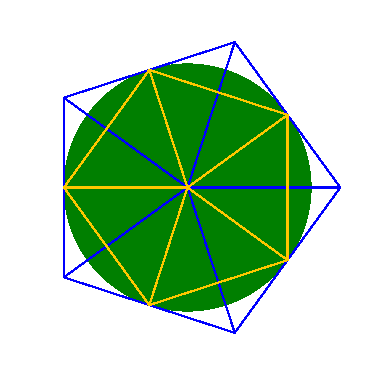
\includegraphics{03archimedes.pdf}}
    \end{picture}


On a historical note: Archimedes managed to compute $A_{96}$ and
$B_{96}$ and by doing this got the most accurate approximation for
$\pi$ that was known in his time.  See also:
\begin{center}
  \url{http://www-history.mcs.st-andrews.ac.uk/HistTopics/Pi_through_the_ages.html}
\end{center}

